\documentclass[tikz,border=6pt]{standalone}
\usepackage{tikz}
\usetikzlibrary{arrows.meta,positioning}
\definecolor{nebula}{HTML}{6366F1}
\definecolor{spark}{HTML}{14B8A6}
\definecolor{ink}{HTML}{334155}
\begin{document}
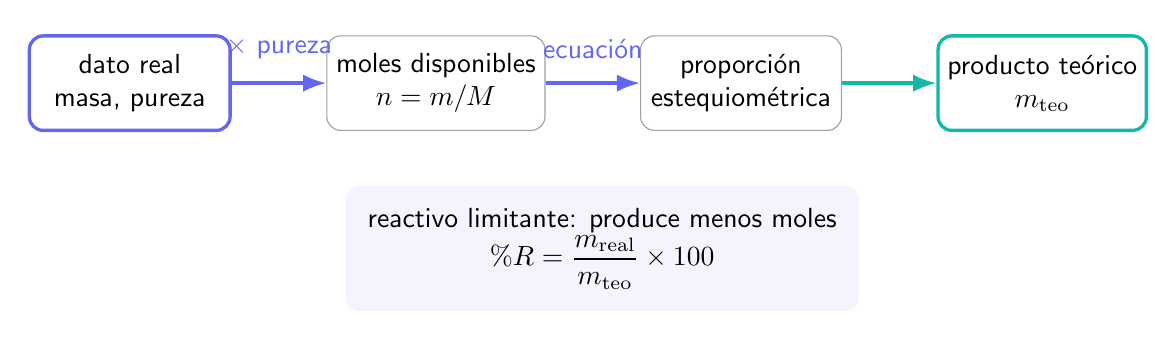
\begin{tikzpicture}[font=\sffamily,>=Latex,node distance=1.2cm,box/.style={draw=ink!50,rounded corners=5pt,minimum width=2.55cm,minimum height=1.2cm,align=center,fill=white}]
  \node[box,draw=nebula,very thick] (data) {dato real\\masa, pureza};
  \node[box,right=of data] (moles) {moles disponibles\\$n=m/M$};
  \node[box,right=of moles] (ratio) {proporci\'on\\estequiom\'etrica};
  \node[box,right=of ratio,draw=spark,very thick] (product) {producto te\'orico\\$m_{\rm teo}$};
  \draw[->,very thick,nebula] (data)--(moles) node[midway,above=5pt] {$\times$ pureza};
  \draw[->,very thick,nebula] (moles)--(ratio) node[midway,above=5pt] {ecuaci\'on};
  \draw[->,very thick,spark] (ratio)--(product);
  \node[align=center,fill=nebula!7,rounded corners=5pt,inner sep=8pt] at (6,-2.1) {reactivo limitante: produce menos moles\\$\displaystyle \%R=\frac{m_{\rm real}}{m_{\rm teo}}\times100$};
\end{tikzpicture}
\end{document}
